\documentclass[uct_visualisation_thesis.tex]{subfiles}

\section{Architektura i działanie systemu}
\subsection{Wykorzystane technologie}
W naszym projekcie zdecydowaliśmy się skorzystać z technologii wymienionych poniżej.
\begin{enumerate}
	\item Języka \textit{Python} w wersji 3.7.2, który jest udostępniany na licencji \textit{GNU General Public License}.
	\item Biblioteki \textit{VisPy} w wersji 0.6.3, która udostępnia komponenty związane z wizualizacją graficzną. Wykorzystujemy tę bibliotekę w połączeniu z \textit{OpenGL} w wersji 2.1. Biblioteka \textit{VisPy} jest stworzona w oparciu o licencję \textit{BSD}, co w kontekście projektu na pracę inżynierską pozwala na modyfikowanie i wykorzystywanie jej.
	\item Biblioteki \textit{NumPy} w wersji  1.18.1, która odpowiada za wydajne operacje na macierzach. Zgodnie z umową licencyjną opisaną przez autorów \textit{NumPy}, można wykorzystywać ich narzędzie w zakresie pracy naukowej.
	\item Nakładki na bibliotekę \textit{Qt} - \textit{PyQt} w wersji 5.9.2. \textit{PyQt} umożliwia tworzenie interfejsu graficznego. Dla projektów takich jak praca inżynierska, \textit{PyQt} dystrybuowana jest na zasadach \textit{GNU General Public License}.
	\item Biblioteki \textit{fman build system (fbs)} w wersji 0.8.4, ułatwiającej pakowanie aplikacji korzystających z biblioteki \textit{PyQt}. To oprogramowanie dystrybuowane jest na zasadach \textit{GNU General Public License}.
	\item Narzędzia \textit{pdoc} w wersji 0.3.2, służącego do automatycznego generowania dokumentacji aplikacji. Zgodnie z umową licencyjną opisaną przez autorów \textit{pdoc}, można wykorzystywać ich narzędzie bez ograniczeń.
\end{enumerate}


\subsection{Wstęp}
Aplikacja jest podzielona na pięć oddzielnych modułów: \textit{Algorytm}, \textit{Serializacja}, \textit{Wizualizacja}, \textit{Gry}, które będą funkcjonować w obrębie nadrzędnego modułu - \textit{Aplikacji głównej}. Cele każdego z modułów i zadania powierzone im są przedstawione w rozdziałach \ref{subsec:algorithm} - \ref{subsec:mainapp}.


\subsection{Algorytm} \label{subsec:algorithm}
Moduł \textit{Algorytm} jest implementacją metody MCTS, korzystającą z wariantu UCT. Odpowiedzialnością tego modułu jest wyznaczanie kolejnego ruchu na podstawie dostarczonego stanu gry. Opisywany moduł będzie odpowiadał za iteracyjne tworzenie drzewa stanów i przeszukiwanie go w celu wyznaczenia najbardziej korzystnego ruchu. Użytkownik będzie miał możliwość zmiany liczby iteracji algorytmu albo ograniczenie czasowe jego działania.\\

W listingu \ref{lst:mcts}, opisującym zaimplementowany algorytm, operujemy na trzech istotnych zmiennych - \textit{tree}, \textit{curr\textunderscore node} i \textit{curr\textunderscore state}. Odpowiedzialnością struktury opisującej drzewo - \textit{tree} - jest przechowywanie korzenia oraz stanu wyjściowego rozgrywki, który jest tej samej struktury co zmienna \textit{curr\textunderscore state}. Struktura opisująca wierzchołek - \textit{curr\textunderscore node} - przechowuje wszystkie informacje na temat wierzchołka drzewa, wraz z referencjami do wierzchołków potomnych i rodzica. Dokładne relacje między komponentami zostały opisane na diagramie \ref{rys:umldiagram}.


\subsection{Serializacja}
\textit{Serializacja} jest modułem odpowiadającym za zapisywanie drzew do plików formacie binarnym lub csv. Oba schematy są rekurencyjne, bo taka jest również struktura generowanych przez aplikację drzew. To oznacza, że w celu zapisania całego drzewa, wystarczy przekazać odpowiednim komponentom jego korzeń.\\

\textbf{\large Serializacja binarna} \\
W serializacji binarnej przyjmujemy opisany niżej schemat.

\begin{itemize}
	\item \textbf{liczba całkowita} - wartość liczby zakodowanej w U2 na 4 bajtach. Bajty liczby w kolejności little endian.
	\item \textbf{napis}:
	\begin{itemize}
		\item liczba bajtów w napisie \textit{(liczba całkowita)},
		\item zawartość napisu kodowana w UTF8.
	\end{itemize}
	\item \textbf{liczba zmiennoprzecinkowa} - wartość liczby zakodowanej w IEEE754 na 64 bitach w kolejności little endian.
	\item \textbf{wierzchołek:}
	\begin{itemize}
		\item nazwa stanu \textit{(napis)},
		\item $m$ - liczba węzłów potomnych \textit{(liczba całkowita)},
		\item $m$ powtórzeń następującego bytu:
		\begin{itemize}
			\item nazwa ruchu \textit{(napis)},
			\item licznik odwiedzin \textit{(liczba całkowita)},
			\item dodatkowy licznik odwiedzin \textit{(liczba całkowita)},
			\item średnia wypłata \textit{(liczba zmiennoprzecinkowa)},
			\item węzeł potomny \textit{(wierzchołek)}.
		\end{itemize}
	\end{itemize}
\end{itemize}


\textbf{\large Serializacja do plików csv} \\
W serializacji do plików csv przyjmujemy, że każdy kolejny wiersz odpowiada kolejnemu wierzchołkowi drzewa, a kolejne wartości opisujące wierzchołek oddzielamy przecinkami. Ostatnią wartością jest liczba wierzchołków potomnych. Każdy wierzchołek serializujemy do wiersza postaci:

\begin{center}
	\textbf{R, O, O2, W, S, D}
\end{center}
Oznaczenia:
\begin{itemize}
	\item R - nazwa ruchu,
	\item O - licznik odwiedzin,
	\item O2 - dodatkowy licznik odwiedzin,
	\item W - średnia wypłata algorytmu za ruch,
	\item S - nawa stanu,
	\item D - liczba wierzchołków potomnych.
\end{itemize}

Kolejność wierszy opisujących wierzchołki jest analogiczna do odwiedzania wierzchołków przez algorytm przeszukiwania drzewa wgłąb, począwszy od korzenia.

\begin{itemize}
	\item Jeśli wierzchołek $v$ ma jednego potomka $v_1$, to wiersz opisujący $v_1$ znajduje się pod wierszem opisującym $v$.
	\item Jeśli wierzchołek $v$ ma $n$ potomków $v_1, v_2, ..., v_n$ i żaden z potomków nie ma swoich potomków, to pod wierszem opisującym $v$ kolejne $n$ wierszy opisuje wierzchołki $v_1, v_2, ..., v_n$.
\end{itemize}


\subsection{Wizualizacja}
Moduł \textit{Wizualizacja} udostępnia funkcjonalność wizualizacji dostarczonych drzew. \textit{Wizualizacja} jest jedynym modułem, który korzysta z technologii \textit{VisPy} oraz \textit{NumPy}. Wykorzystanie tych technologii ma na celu odpowiednio wydajne wyświetlenie wizualizacji oraz przechowywanie wektorów z danymi, które będzie można przekazać karcie graficznej. Zadania \textit{Wizualizacji} są wymienione poniżej.

\begin{itemize}
	\item Przypisanie wierzchołkom drzewa miejsce na płaszczyźnie przy użyciu usprawnionego algorytmu Walkera i przetransformowanie wyznaczonych koordynatów do układu współrzędnych OpenGL.
	\item Przypisanie krawędziom koloru w zależności od liczby odwiedzin wierzchołka.
	\item Przypisanie wierzchołkom koloru w zależności od gracza reprezentowanego stanu gry.
	\item Detekcja kliknięcia wierzchołka przez użytkownika.
	\item Wyświetlenie drzewa.
	\item Przybliżanie, oddalanie i poruszanie się po wizualizacji.
\end{itemize}


\subsection{Gry}
Prezentowane rozwiązanie udostępnia dwie gry planszowe w ramach modułu \textit{Gry}. System został przygotowany z myślą o rozszerzaniu o kolejne gry. Wymagania, które należy spełnić, dodając kolejną grę, są opisane w rozdziale \ref{subsec:uml}.


\subsection{Aplikacja główna} \label{subsec:mainapp}
\textit{Aplikacja główna} jest modułem łączącym wszystkie pozostałe. Ten moduł skupia się na zaprezentowaniu funkcjonalności wszystkich modułów w formie aplikacji okienkowej. Interfejsy, które udostępnia \textit{Aplikacja główna}, są opisane w rozdziale \ref{sec:ui}.


\section{Główne komponenty aplikacji}
\subsection{Diagram klas} \label{subsec:uml}

\begin{figure}[h!]
	\centering
	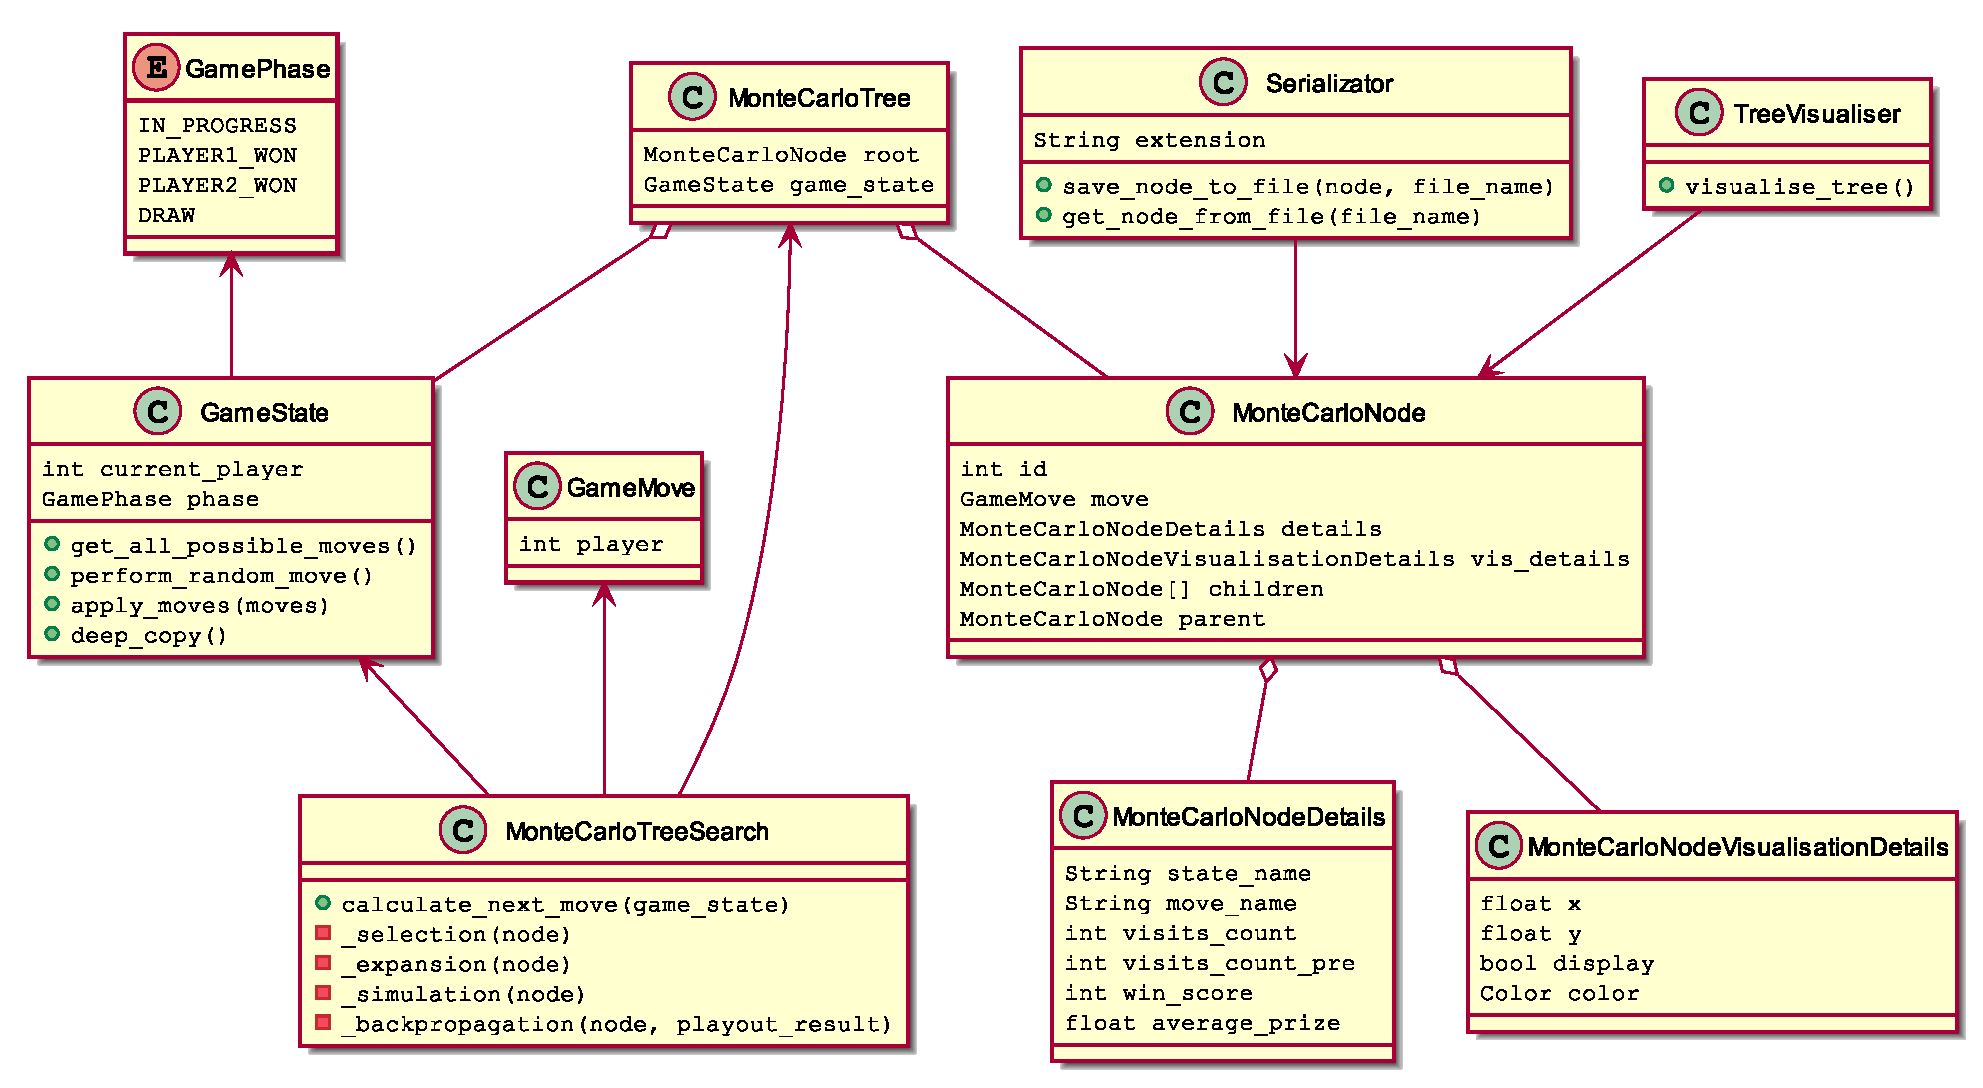
\includegraphics[width=\linewidth]{umldiagram}
	\caption{Diagram UML głównych komponentów aplikacji}
	\label{rys:umldiagram}
\end{figure}

Zgodnie z diagramem \ref{rys:umldiagram}, klasy \textit{MonteCarloTreeSearch}, \textit{TreeVisualiser} oraz \textit{Serializator} są pośrednio lub bezpośrednie zależne od klasy \textit{MonteCarloNode}, opisującej wierzchołek w drzewie. Jest to część wspólna modułów \textit{Algorytm}, \textit{Wizualizacja} i \textit{Serializacja}. Klasa \textit{MonteCarloNode} przechowuje referencję do swojego rodzica oraz wierzchołków potomnych, aby zachować rekurencyjną strukturę drzewa.\\

Metoda \textit{calculate\textunderscore next\textunderscore move} klasy \textit{MonteCarloTreeSearch} odpowiada za wykonanie kolejnych iteracji algorytmu. Algorytm zapisuje informacje o rozgrywanych playoutach w polach klasy \textit{MonteCarloNodeDetails} analizowanych wierzchołków. Ruch oraz stan analizowanej gry są opisane odpowiednio przez klasy \textit{GameMove} i \textit{GameState}. Implementacja metod tych klas daje możliwość łatwego rozszerzenia aplikacji o inne gry. Istotny z punktu widzenia konstrukcji drzewa jest stan rozgrywki, który opisują pola typu wyliczeniowego \textit{GamePhase}.\\

\textit{TreeVisualiser} jest głównym komponentem modułu \textit{Wizualizacja}. Jego odpowiedzialnością jest wyznaczenie układu wierzchołków drzewa na płaszczyźnie oraz wyświetlenie wygenerowanej wizualizacji. Szczegóły związane z rysowaniem każdego wierzchołka, takie jak jego współrzędne czy kolor, zawarte są w polach klasy \textit{MonteCarloVisualisationDetails}.\\

\textit{Serializator} jest klasą opisującą funkcjonalności, które mają udostępnić właściwe implementacje serializatorów, czyli serializowanie drzew do plików oraz deserializację z plików.


\section{Interfejs użytkownika} \label{sec:ui}
\subsection{Wstęp}
Graficzny interfejs użytkownika składać się będzie z trzech głównych okien, a logika jego działania będzie w całości zawarta w module \textit{Aplikacja główna}. Zadaniem graficznego interfejsu jest umożliwienie uruchomienia poszczególnych modułów użytkownikom końcowym.

\subsection{Menu główne}
Ukazane na rysunku \ref{rys:main_menu} menu główne będzie głównym oknem aplikacji i będzie to pierwsza rzecz, którą zobaczy użytkownik po uruchomieniu programu.
\begin{figure}[h!]
	\centering
	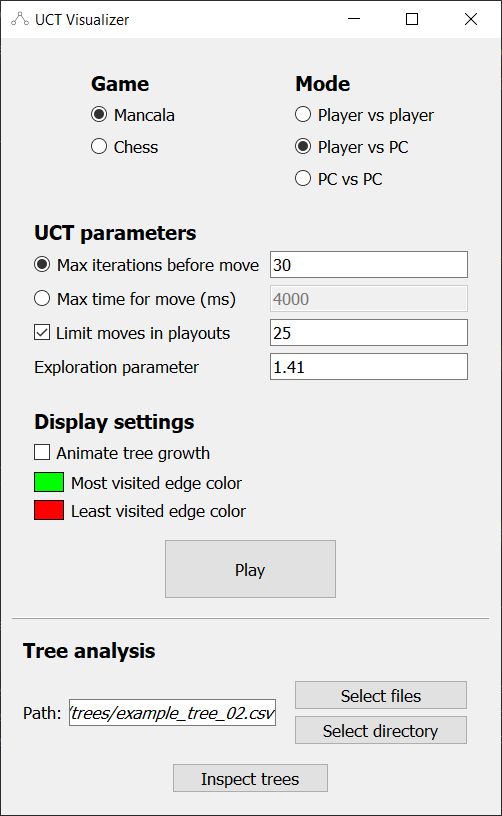
\includegraphics[width=0.55\textwidth]{okno-glowne}
	\caption{Okno menu głównego}
	\label{rys:main_menu}
\end{figure}

\noindent Dwa moduły, do których można przejść z tego okna, to rozgrywka i analiza drzewa.	Żeby rozegrać grę, należy nacisnąć na przycisk \textit{Play}. Powyżej znajdować się będzie szereg opcji, który pozwoli użytkownikowi ustawić parametry gry dostosowane do jego preferencji:
\begin{itemize}
	\item \textbf{wybór gry} -- do dyspozycji gracza oddane są dwie gry -- szachy i mankala,
	\item \textbf{wybór trybu rozgrywki} -- użytkownik może wybrać jeden z trzech dostępnych trybów gry:
	\begin{itemize}
		\item \textbf{dwóch graczy} -- tryb bez udziału algorytmu UCT, a co za tym idzie, również bez wizualizacji,
		\item \textbf{gracz przeciwko PC} -- w tym trybie gracz ma okazję zmierzyć się z komputerem, oglądając przy tym generowane drzewa stanów algorytmu UCT,
		\item \textbf{PC przeciwko PC} -- rozgrywka komputera z samym sobą, z możlwiością analizowania wynikowych drzew stanów algorutmu. Wybór tego trybu oznacza brak możliwości wykonywania samodzielnych ruchów przez użytkownika, jednakże to od niego będzie zależało, kiedy algorytm wykona kolejny ruch -- będzie miał do dyspozycji przycisk, za pomocą którego będzie mógł powodować postęp w rozgrywce. 
	\end{itemize}
	\item \textbf{wybór liczby iteracji algorytmu} -- liczba powtórzeń wykonania przez algorytm czterofazowej tury metody MCTS opisanej w rozdziale 3.3.1,
	\item \textbf{wybór maksymalnego czasu} -- podany w milisekundach; czas, po którym komputer będzie przerywał obliczenia i wykona ruch,
	\item \textbf{ustawienie limitu ruchów} -- opcjonalne pole, w którym użytkownik może ustalić maksymalną liczbą ruchów w fazie symulacji algorytmu UCT, w celu wcześniejszego kończenia niepożądanie długich rozgrywek,
	\item \textbf{ustalenie wartości parametru eksploracji} -- im większy, tym chętniej algorytm UCT będzie wybierał rzadziej odwiedzane ruchy. Domyślnie $\sqrt{2}$,
	\item \textbf{animowanie rozrostu drzewa} -- wybór tej opcji sprawia, że drzewo stanów algorytmu zostaje wyświetlone nie tylko po każdym wykonanym ruchu przez komputer, ale też po każdej iteracji.
	\item \textbf{wybór kolorów krawędzi drzewa} - po kliknięciu na któryś z widocznych kolorów ukaże się paleta systemowa, z której można wybrać inne kolory krawędzi. Najczęściej i najrzadziej odwiedzane węzły drzewa przyjmą wskazane przez użytkownika kolory, inne zaś --- kolory z ich gradientu, proporcjonalnie do wartości skrajnych licznika odwiedzin.
\end{itemize}

Drugą kluczową opcją dostępną z menu głównego aplikacji jest możlwiość przejścia do okna analizy drzewa lub sekwencji drzew. Jest ona dostępna po naciśnięciu przycisku \textit{Inspect trees}. Użytkownik może wczytać pliki z dysku na dwa sposoby: wybierając pliki z folderu bezpośrednio lub wybierając cały katalog, w którym się one znajdują. Do tego celu służą osobno dwa przyciski: \textit{Select files} i \textit{Select directory}, które znajdują się na prawo od pola tekstowego, w którym wyświetlana jest pełna ścieżka do aktualnie wybranego pliku lub katalogu. W przypadku wybrania większej ilości plików, pokazywana jest ich liczba.
Można jednocześnie wybierać pliki w formacie CSV i binarnym (.tree), których sposób kodowania jest opisany dokładniej w rozdziałach xx i yy.
W przypadku wybrania nieprawidłowego katalogu lub niepoprawnych plików, na ekranie użytkownika pojawi się błąd informujący o problemie, który nastąpił.

\subsection{Analiza drzewa}
W oknie ukazanym na rysunku \ref{rys:analyze_tree} będziemy mogli oglądać wczytane lub wygenerowane drzewa. 
\begin{figure}[h!]
	\centering
	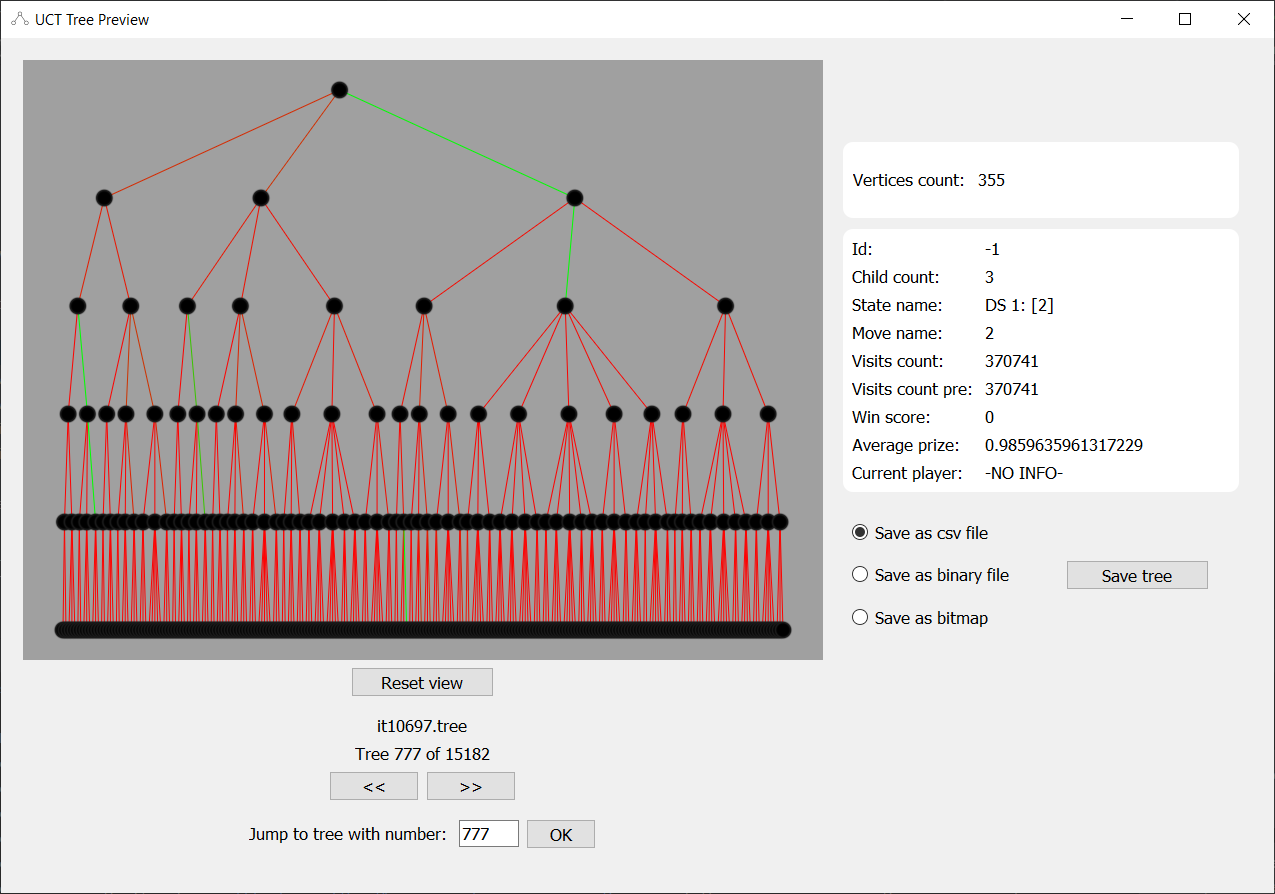
\includegraphics[scale=0.57]{okno-analiza}
	\caption{Okno analizy drzewa}
	\label{rys:analyze_tree}
\end{figure}

Kluczową funkcją będzie tutaj możliwość dynamicznego przybliżania i oddalania go (za pomocą przycisków plusa i minusa na ekranie lub scrolla) wraz z możliwością klikania poszczególnych węzłów w celu pozyskania stanu rozgrywki w danym momencie. Widoczna będzie także informacja o tym, ile razy algorytm odwiedził dany węzeł, ile razy doprowadził on do wygranej oraz średnią nagrodę za ruch w danym węźle. Możliwe będzie też wycentrowanie oglądanego drzewa.

W przypadku wczytania większej ilości drzew będzie możliwość przełączania ich za pomocą przycisków ze strzałkami w lewo i w prawo. Zaznaczane wtedy będą różnice w węzłach i krawędziach względem poprzedniego drzewa.

\subsection{Rozgrywka}
Poniżej przedstawiony jest przykładowy interfejs graficzny, do którego użytkownik będzie miał dostęp podczas rozgrywki.
\begin{figure}[h!]
	\centering
	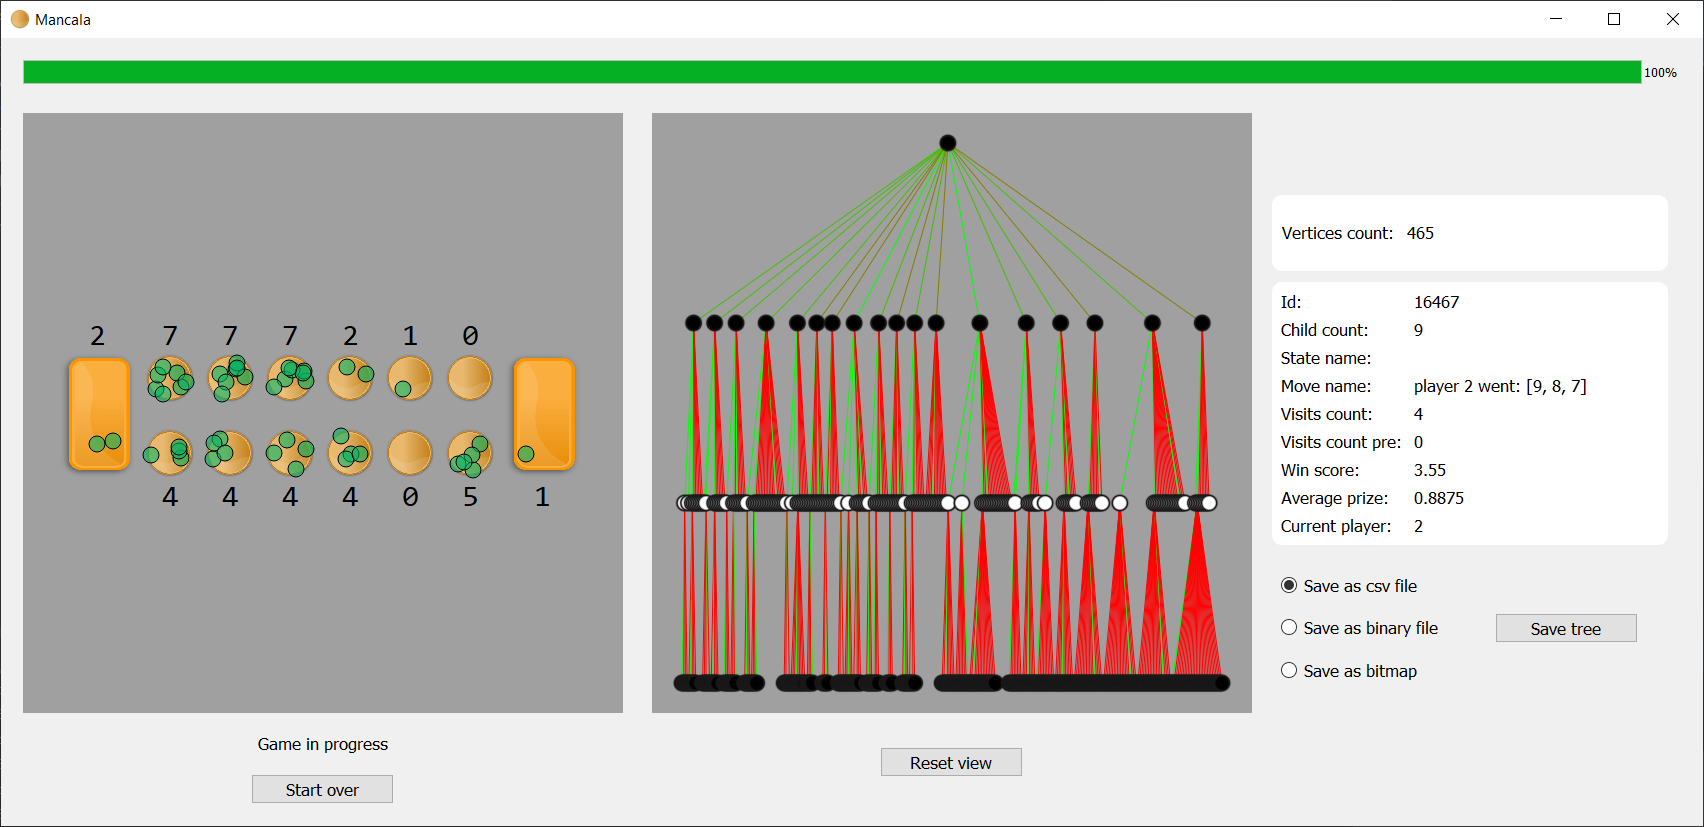
\includegraphics[width=1\textwidth]{okno-mancala}
	\caption{Okno rozgrywki}
	\label{rys:game_view}
\end{figure}

Zgodnie z projektem okna przedstawionym na rysunku \ref{rys:game_view}, widok rozgrywki będzie podzielony na dwie części. Gra zawierać się będzie w wyżej pokazanym oknie po lewej stronie. To tutaj użytkownik za pomocą przygotowanego do gier GUI będzie mógł wykonać ruch. W prawej części okna znajdować się będą opcje związane z aktualnym stanem rozgrywki, między innymi:

\begin{itemize}
	\item informacja o aktualnym stanie gry.
	\item wykonaj kolejny ruch - wyłącznie w trybie rozgrywki maszyna kontra maszyna. Użytkownik będzie miał możliwość kontrolowania wykonywanych przez komputer ruchów, aby samemu móc powodować postęp w rozgrywce.
	\item przeanalizuj wygenerowane drzewa - będzie to przycisk otwierający drugie okno z opisaną wcześniej analizą drzewa. Nad przyciskiem znajduje się parametr mówiący ile ruchów wstecz użytkownik ma zamiar analizować. Jedno drzewo będzie odpowiadać jednemu ruchowi komputera, a jako pierwsze wyświetli się drzewo przedstawiające stan z ostatniego ruchu i reszta będzie odpowiednio w kolejności chronologicznej (od końca).
	\item wyeksportuj drzewo do pliku (csv, png lub binarnego).
\end{itemize}